\chapter{Evaluations}
\section{Industrial evaluation: Oberthur}
\section{Industrial evaluation: Axalto}
\section{Bytecode Verifier}
The tools have also been tested on a bytecode verifier java implementation. A termination proof has been provided.
A specific implementation has been coded with on one hand the main loop which remain unchanged whatever the specifications of the virtual machine Java chosen, and other instructions and memory states which depends on selected model.
The main loop is in a package which contains abstract classes: 
the instructions and the states are implemented in a more generic way.
The package containing the implementation is composed from the instructions for the standard Java types and of the states of memory typing. 
\subsection {Memory states}
The memory states are represented by the State class, which is an abstract class.  It does not contain any precise definition of the memory: 
one has no information on the stack or on the local variables table. 
The implementation is relatively simple: 
it is a class which contains a type stack and a table of the types of the local variables. 
Functions allowing to read simply these structures and to generate verification error in the cases of misuse are defined.   
\subsection{Instructions}
The instructions are also represented by an abstract class: 
the class Instruction.  
Since in the Kildall algorithm each instruction is associated to a memory state,  the Instruction class has a field of the State type. 
An instruction can also have one or more successors. 
This relation is represented by a field which is the list of the successors of the instruction.  
One of the other aspects is the fact that on associate to each instruction a boolean field to determine if it has been modified or not.

Several propreties of the bytecode verifier are for;alised in this class.
First of all one verifies that the successors of the instruction are well included in the others instructions of the program. 
If these successors pointed towards external instructions, an verification error would be returned. 

The others important properties concern the pure function {\tt buildNewState}.
This function builds the typing state of the execution of an instruction  on the current state.
This construction can fail if the instruction tries for example to pop an element when the stack is empty.
If it succeeds, a new non null state is build.

Around ten instructions have been implementeds:  {\tt load} and {\tt blind} for the access to local variables, {\tt push} and {\ ttpop}   to obtain or put element on the stack, {\tt op1} and {\ ttop2} which is two operators who consume both the two top element of the stack and which replaces them by a eesultat of a certain type, {\tt ifle} and {\tt jump} instructions of jump towards another instruction successor, {\tt nop}  the instruction which does not do anything   and finally {\tt stop} which is an instruction which does not have a successor.
These instructions have an associated type in the OperandType class,
who can be None, Type1 or Type2.  Those are the minimal instructions to have a Java-like program.  
\subsection {The main loop}
The main loop is implementes in the Verifier class.
It is not an abstract class because it uses the properties of the State and Instruction abstract classes  to verify an instruction set on particular states.
This class provides two functions, the function  {\ tt verify} in which the loop is written and the function {\ tt check} which verify an instruction.

%The m \ 'ethode check ensures that all \ 'states of the successors of an instruction donn \ 'ee,    are larger or \ 'equal that the \ 'states before the ex \ 'ecution of the m \ 'ethode. This   propri \ 'and \ 'E seems simple \ `has to express but it implies several Pr \ 'erequis.  First of all it should be guaranteed that the successors of the instructions point all worms of   valid instructions. Then that all the instructions are diff \ 'erentes of no one and that theirs  \ 'states are too diff \ 'erents of no one them.    The Pr \ calculation weaker 'econdition of Jack forces us \ `has to add these propri \ 'and \ 'be    Li \ 'ees \ `with the S \ 'emantic of the language Java.  .   %Pour to facilitate the evidence I have \ 'and \ 'E oblig \ 'E  %de to add a certain number of assertions.    

The {\ tt verify} method is the main loop of the bytecode verifier.
It contains two nested loops. 
The internal one is a {\tt for} loop which iterates on the instructions  and verify all the quoted instructions (as described in the Kildall algorithm). 
The termination of the internal loop is easy to prove.
The {\tt for} loop executes as many time as there are numbers in the table.
The external {\tt while} loop stops the algorithm when no more instruction typing state is modified.
This termination is not obvious to prove, especially with JML, since it only allow to prove loop termination by giving an integer variant.

Since the states have to be used to show the algorithm termination,  
one has to make correspond each state  with an integer. 
Thus at each loop iteration, the integer associated with the state either increase or preserve the same value; and it exists a maximum value.


\begin{figure}[ht]  
\begin{center}    
\begin{tabular}{p {0.4 \textwidth} c c c c}  
{\bf Classes:} & State & Instruction & Verifier \\  
{\bf Lines of code:} & 14 & 47 & 66 \\  
{\bf Lines of annotations:} & 20 & 54 & 81 \\  \raggedright 
{\bf Proof obligations:} & 26 & 129 & 627 \\  \raggedright 
{\bf Automatically proved proof obligations:} & 17 & 93 & 112 \\  
{\bf Average length of a non-automatic proof:} & 3 & 6 & 12 \\    
\end{tabular}  
\end{center}  
\caption{Some statistics on proof}  
\label{stats}  
\end{figure}    
\subsection{Proofs}
The first proofs are relatively easy. 
The State class is proven almost automatically; 
except for the constructor where it is necessary to break a disjunction ({\tt instance S $\vee$ S = null}) to prove the invariants.

The Instruction class has also been relatively easy to prove. 
A significant number of proof was done automatically (approximately 90 \%); 
then majority of proof could be trivially resolved, except some lemma concerning  a loop termination.    

Finally the Verifier class was harder to prove.
The lemmas were containing too many hypotheses to be automatically proved.
Around 500 proof obligations have to be resolved manually.
Some of them was obvious and were resolved with quite the same script, but the script cannot be automated.
Some of them was complex: the proof script became little large (an average of 30 steps).
The lemmas conerning the loop invariant of the verify method and its initialisation were the most difficult.
\section{Low-Footprint Java-to-Native Compilation}
% Pertinence of compiling bytecode into native code for embedded devices
Enabling Java on embedded and restrained systems is an important challenge for today's industry and research groups~\cite{Mulchandani1998}. Java brings features like execution safety and low-footprint program code that make this technology appealing for embedded devices which have obvious memory restrictions, as the success of Java Card witnesses. However, the memory footprint and safety features of Java come at the price of a slower program execution, which can be a problem when the host device already has a limited processing power. As of today, the interest of Java for smart cards is still growing, with next generation operating systems for smart cards that are closer to standard Java systems~\cite{Lagosanto2002,Grimaud2003}, but runtime performance in still an issue. To improve the runtime performances of Java systems, a common practice is to translate some parts of the program bytecode into native code.

% Cost of native code
Doing so removes the interpretation layer and improves the execution speed, but also greatly increases the memory footprint of the program: it is expected that native code is about three to four times the size of its Java counterpart, depending on the target architecture. This is explained by the less-compact form of native instructions, but also by the fact that many safety-checks that are implemented by the virtual machine must be reproduced in the native code. For instance, before dereferencing a pointer, the virtual machine checks whether it is \texttt{null} and, if it is, throws a \texttt{NullPointerException}. Every time a bytecode that implements such safety-behaviors is compiled into native code, these behaviors must be reproduced as well, leading to an explosion of the code size. Indeed, a large part of the Java bytecode implement these safety mechanisms.

% Usefulness of runtime checks
Although the runtime checks are necessary to the safety of the Java virtual machine, they are most of the time used as a protection mechanism against programming errors or malicious code: A runtime exception should be the result of an exceptional, unexpected program behavior and is rarely thrown when executing sane code - doing so is considered poor programming practice. The safety checks are therefore without effect most of the time, and, in the case of native code, uselessly enlarge the code size.

% Our contribution
Several studies proposed to factorize these checks or in some case to eliminate them, but none proposed a complete elimination without hazarding the system security. In this paper, we use formal proofs to ensure that run-time checks can never be true into a program, which allows us to completely and safely eliminate them from the generated native code. The programs to optimize are JML-annotated against runtime exceptions and verified by the Java Applet Correctness Kit (JACK~\cite{BRL-JACK}). We have been able to remove almost all of the runtime checks on tested programs, and obtained native ARM thumb code which size was comparable to the original bytecode.

\subsection{Java and Ahead-of-Time Compilation}
\label{sec:sota}

Compiling Java into native code common on embedded devices. This section gives an overview of the different compilation techniques of Java programs, and points out the issue of runtime exceptions.

\subsubsection{Ahead-of-Time \& Just-in-Time Compilation}

% JIT & AOT compilations
Ahead-of-Time (AOT) compilation is a common way to improve the efficiency of Java programs. It is related to Just-in-Time (JIT) compilation by the fact that both processes take Java bytecode as input and produce native code that the architecture running the virtual machine can directly execute. AOT and JIT compilation differ by the time at which the compilation occurs. JIT compilation is done, as its name states, just-in-time by the virtual machine, and must therefore be performed within a short period of time which leaves little room for optimizations. The output of JIT compilation is machine-language. On the contrary, AOT compilation compiles the Java bytecode way before the program is run, and links the native code with the virtual machine. In other words, it translates non-native methods into native methods (usually C code) prior to the whole system execution. AOT compilers either compile the Java program entirely, resulting in a 100\% native program without a Java interpreter, or can just compile a few important methods. In the latter case, the native code is usually linked with the virtual machine. AOT compilation have no or few time constraints, and can generate optimized code. Moreover, the generated code can take advantage of the C compiler's own optimizations.

% Why JIT is not applicable to embedded devices
JIT compilation in interesting by several points. For instance, there is no prior choice about which methods must be compiled: the virtual machine compiles a method when it appears that doing so is beneficial, e.g. because the method is called often. However, JIT compilation requires embedding a compiler within the virtual machine, which needs resources to work and writable memory to store the compiled methods. Moreover, the compiled methods are present twice in memory: once in bytecode form, and another time in compiled form. While this scheme is efficient for decently-powerful embedded devices such as PDAs, it is inapplicable to very restrained devices like smartcards or sensors. For them, ahead-of-time compilation is usually preferred because it does not require a particular support from the embedded virtual machine outside of the ability to run native methods, and avoids method duplication. AOT compilation has some constraints, too: the compiled methods must be known in advance, and dynamically-loading new native methods is forbidden, or at least very unsafe.

% Runtime exceptions
Both JIT and AOT compilers must produce code that exactly mimics the behavior of the Java virtual machine. In particular, the safety checks performed on some bytecode must also be performed in the generated code.

\subsubsection{Java Runtime Exceptions}
\label{sec:runtimeexceptions}
% Why runtime exceptions
The JVM (Java Virtual Machine)~\cite{VMSpec} specifies a safe execution environment for Java programs. Contrary to native execution, which does not automatically control the safety of the program's operations, the Java virtual machine ensures that every instruction operates safely. The Java environment may throw predefined runtime exceptions at runtime, like the following ones:

If the JVM detects that executing the next instruction will result in an inconsistency or an illegal memory access, it throws a runtime exception, that may be caught by the current method or by other methods on the current stack. If the exception is not caught, the virtual machine exits. This safe execution mode implies that many checks are made during runtime to detect potential inconsistencies. 

Of the 202 bytecodes defined by the Java virtual machine specification, we noticed that 43 require at least one runtime exception check before being executed. While these checks are implicitly performed by the bytecode interpreter in the case of interpreted code, they must explicitly be issued every time such a bytecode is compiled into native code, which leads to a code size explosion. Ishizaki et al. measured that bytecodes requiring runtime checks are frequent in Java programs: for instance, the natively-compiled version of the SPECjvm98 \texttt{compress} benchmark has 2964 exception check sites for a size of 23598 bytes. As for the \texttt{mpegaudio} benchmark, it weights 38204 bytes and includes 6838 exception sites~\cite{Ishizaki1999}. The exception check sites therefore make a non-neglectable part of the compiled code.

\subsection{Optimizing Ahead-of-Time Compiled Java Code}
\label{sec:method}

%verification procedure
Verifying that a bytecode program does not throw Runtime exceptions using JACK involves several stages:
\begin{enumerate}
\item writing the JML specification at the source level of the application, which expresses that no runtime exceptions are thrown.
\item compiling the Java sources and their JML specification\footnote{the BML specification is inserted in user defined attributes in the class file and so does not violate the class file format}.
\item generating the verification conditions over the bytecode and its BML specification, and proving the verification conditions~\ref{proofs}. During the calculation process of the verification conditions, they are indexed with the index of the instruction in the bytecode array they refer to and the type of specification they prove (e.g. that the proof obligation refers to the exceptional postcondition in case an exception of type \texttt{Exc} is thrown when executing the instruction at index \texttt{i} in the array of bytecode instructions of a given method). Once the verifications are proved, information about which instructions can be compiled without runtime checks is inserted in user defined attributes of the class file.
\item using these class file attributes in order to optimize the generated native code. When a bytecode that has one or more runtime checks in its semantics is being compiled, the bytecode attribute is checked in order to make sure that the checks are necessary. It indicates that the exceptional condition has been proved to never happen, then the runtime check is not generated.
\end{enumerate}

Our approach benefits from the accurateness of the JML specification and from the bytecode verification condition generator. Performing the verification over the bytecode allows to easily establish a relationship between the proof obligations generated over the bytecode and the bytecode instructions to optimized.

In the rest of this section, we explain in detail all the stages of the optimization procedure.

\subsubsection{Methodology for Writing Specification Against Runtime Exception}

We now illustrate with an example which annotations must be generated in order to check if a method may throw an exception. Figure~\ref{fig:jmlexample}\footnote{although the analysis that we describe is on bytecode level, for the sake of readability, the examples are also given on source level} shows a Java method annotated with a JML specification. The method \verb!clear! declared in class \verb!Code_Table! receives an integer parameter \verb!size! and assigns \verb!0! to all the elements in the array field \verb!tab! whose indexes are smaller than the value of the parameter \verb!size!. The specification of the method guarantees that if every caller respects the method precondition and if every execution of the method guarantees its postcondition then the method \verb!clear! never throws an exception of type or subtype \verb!java.lang.Exception!\footnote{Note that every Java runtime exception is a subclass of \texttt{java.lang.Exception}}. This is expressed by the class and method specification contracts.
First, a class invariant is declared which states that once an instance of type \verb!Code_Table! is created, its array field \verb!tab! is not null. The class invariant guarantees that no method will throw a \verb!NullPointerException! when dereferencing (directly or indirectly) \verb!tab!.

\begin{figure}
\begin{verbatim}
final class Code_Table {
  private/*@spec_public */short tab[];

  //@invariant tab != null;

  ...

  //@requires size <= tab.length;
  //@ensures true;
  //@exsures (Exception) false;
  public void clear(int size) {
  1  int code;
  2  //@loop_modifies code, tab[*];
  3  //@loop_invariant code <= size && code >= 0;
  4  for (code = 0; code < size; code++) {
  5    tab[code] = 0;
     }
  }
}
\end{verbatim}

\caption{\sc A JML-annotated method}
\label{fig:jmlexample}
\end{figure}

The method precondition requires the \verb!size! parameter to be smaller than the length of \verb!tab!. The normal postcondition, introduced by the keyword \verb!ensures!, basically says that the method will always terminate normally, by declaring that the set of final states in case of normal termination includes all the possible final states, i.e. that the predicate \verb!true! holds after the method's normal execution\footnote{Actually, after terminating execution the method guarantees that the first \texttt{size} elements of the array tab will be equal to 0, but as this information is not relevant to proving that the method will not throw runtime exceptions we omit it}. On the other hand, the exceptional postcondition for the exception \texttt{java.lang.Exception} says that the method will not throw any exception of type \texttt{java.lang.Exception} (which includes all runtime exceptions). This is done by declaring that the set of final states in the exceptional termination case is empty, i.e. the predicate \texttt{false} holds if an exception caused the termination of the method. The loop invariant says that the array accesses are between index \verb!0! and index \verb!size - 1! of the array \verb!tab!, which guarantees that no loop iteration will cause a \verb!ArrayIndexOutOfBoundsException! since the precondition requires that \verb!size <= tab.length!.

Once the source code is completed by the JML specification, the Java source is compiled using a normal non-optimizing Java compiler that generates debug information like \textrm{LineNumberTable} and \textrm{LocalVariableTable}, needed for compiling the JML annotations. From the resulting class file and the specified source file, the JML annotations are compiled into BML and inserted into user-defined attributes of the class file. 

For generating the verification conditions, we use a bytecode verification condition generator (vcGen) based on a bytecode weakest precondition calculus~\cite{JBL05MP}. 

\subsubsection{From Program Proofs to Program Optimizations }
\label{proofs}
In this phase, the bytecode instructions that can safely be executed without runtime checks are identified. Depending on the complexity of the verification conditions, Jack can discharge them to the fully automatic prover Simplify, or to the Coq and AtelierB interactive theorem prover assistants.
There are several conditions to be met for a bytecode instruction to be optimized safely -- the precondition of the method the instruction belongs to must hold every time the method is invoked, and the verification condition related to the exceptional termination must also hold.
Once identified, proved instructions can be marked in user-defined attributes of the class file so that the compiler can find them.

\subsubsection{More Precise Optimizations}

\label{section:optimprecise}

As we discussed earlier, in order to optimize an instruction in a method body, the method precondition must be established at every call site and the method implementation must be proved not to throw an exception under the assumption that the method precondition holds. This means that if there is one call site where the method precondition is broken then no instruction in the method body will be optimized.

Actually, the analysis may be less conservative and therefore more precise. We illustrate with an example how
one can achieve more precise results.

Consider the example of figure \ref{fig:jmlpreciseex}. On the left side of the figure, we show source code for method \verb!setTo0! which sets the \verb!buff! array element at index \verb!k! to 0. On the right side, we show the bytecode of the same method. The \texttt{iastore} instruction at index \texttt{3} may throw two different runtime exceptions: \texttt{NullPointerException}, or \texttt{ArrayIndexOutOfBoundException}. For the method execution to be safe (i.e. no Runtime exception is thrown), the method requires some certain conditions to be fulfilled by its callers. Thus, the method's precondition states that the \verb!buff! array parameter must not be null and that the \verb!k! parameter must be inside the bounds of \verb!buff!. If at all call sites we can establish that the \verb!buff! parameter is always different from null, but there are sites at which an unsafe parameter \verb!k! is passed the optimization for \texttt{NullPointerException} is still safe although the optimization for \texttt{ArrayIndexOutOfBoundException} is not possible. In order to obtain this kind of preciseness, a solution is to classify the preconditions of a method with respect to what kind of runtime exception they protect the code from. For our example, this classification consists of two groups of preconditions. The first is related to \texttt{NullPointerException}, i.e. \texttt{buff != null} and the second consists of preconditions related to \texttt{ArrayIndexOutOfBoundException}, i.e. \verb! k >= 0 && k <= buff.length!. Thus, if the preconditions of one group are established at all call sites, the optimizations concerning the respective exception can be performed even if the preconditions concerning other exceptions are not satisfied.

\begin{figure}
\begin{minipage}[b]{0.5\linewidth}
\begin{verbatim}
...

//@requires buff != null;
//@requires k >= 0 ;
//@requires k <= buff.length;
//@ensures true;
//@exsures (Exception) false;
public void setTo0(int k,int[] buff)
{
  buff[k] = 0;
}
\end{verbatim}
\end{minipage}
\hspace{.5cm}
\begin{minipage}[b]{0.4\linewidth}
 \begin{verbatim}
 0 aload_2
 1 iload_1
 2 iconst_0
 3 iastore
 4 return
\end{verbatim}
\end{minipage}
\caption{\sc The source code and bytecode of a method that may throw several exceptions}
\label{fig:jmlpreciseex}
\end{figure}

%\subsection{Experimental Results}
%\label{sec:experiments}

%This section presents an application and evaluation of our method on various Java programs.

%\subsubsection{Methodology}

%We have measured the efficiency of our method on two kinds of programs, that implement features commonly met in restrained and embedded devices. \benchname{crypt} and \benchname{banking} are two smartcard-range applications. \benchname{crypt} is a cryptography benchmark from the Java Grande benchmarks suite, and \benchname{banking} is a little banking application with full JML annotations used in~\cite{BRL-JACK}. \benchname{scheduler} and \benchname{tcpip} are two embeddable system components written in Java, which are actually used in the JITS~\cite{JITSWebsite} platform. \benchname{scheduler} implements a threads scheduling mechanism, where scheduling policies are Java classes. \benchname{tcpip} is a TCP/IP stack entirely written in Java, that implements the TCP, UDP, IP, SLIP and ICMP protocols. These two components are written with low-footprint in mind ; however, the overall system performance would greatly benefit from having them available in native form, provided the memory footprint cost is not too important.

%For every program, we have followed the methodology described in section \ref{sec:method} in order to prove that runtime exceptions are not thrown in these programs. We look at both the number of runtime exception check sites that we are able to remove from the native code, and the impact on the memory footprint of the natively-compiled methods with respect to the unoptimized native version and the original bytecode. The memory footprint measurements were obtained by compiling the C source file generated by the JITS AOT compiler using GCC 4.0.0 with optimization option \texttt{-Os}, for the ARM platform in thumb mode. The native methods sizes are obtained by inspecting the .o file with \texttt{nm}, and getting the size for the symbol corresponding to the native method.

%Regarding the number of eliminated exception check sites, we also compare our results with the ones obtained using the JC virtual machine mentioned in~\ref{sec:relatedwork}, version 1.4.6. The results were obtained by running the \texttt{jcgen} program on the benchmark classes, and counting the number of explicit exception check sites in the generated C code. We are not comparing the memory footprints obtained with the JITS and JC AOT compilers, for this result would not be pertinent. Indeed, JC and JITS have very different ways to generate native code. JITS targets low memory footprint, and JC runtime performance. As a consequence, a runtime exception check site in JC is heavier than one in JITS, which would falsify the experiments. Suffices to say that our approach could be applied on any AOT compiler, and that the most relevant measurement is the number of runtime exception check sites that remains in the final binary - our measurements on the native code memory footprint are just here to evaluate the size impact of exception check sites.

%\subsubsection{Results}
%\label{results}
%Table \ref{tab:nbexcsites} shows the results obtained on the four tested programs. The three first columns indicate the number of check sites present in the bytecode, the number of explicit check sites emitted by JC, and the number of check sites that we were unable to prove useless and that must be present in our optimized AOT code. The last columns give the memory footprints of the bytecode, unoptimized native code, and native code from which all proved exception check sites are removed.

%\begin{table}
%\caption{Number of exception check sites and memory footprints when compiled for ARM thumb}
%\begin{center}
%  \begin{tabular}{|l|r@{\extracolsep{0.2cm}}rrrrr|}
%    \hline
%    \multirow{2}*{Program} & \multicolumn{3}{c}{\# of exception check sites} & \multicolumn{3}{c|}{Memory footprint (bytes)}\\
%    \cline{2-4} \cline{5-7} & Bytecode & ~~~~~~JC & Proven AOT & Bytecode & Naive AOT & Proven AOT\\
%    \hline
%    \benchname{crypt} & 190 & 79 & 1 & 1256 & 5330 & 1592\\
%    \benchname{banking} & 170 & 12 & 0 & 2320 & 5634 & 3582\\
%    \benchname{scheduler} & 215 & 25 & 0 & 2208 & 5416 & 2504\\
%    \benchname{tcpip} & 1893 & 288 & 0 & 15497 & 41540 & 18064\\
%    \hline
%  \end{tabular}
%\end{center}
%\label{tab:nbexcsites}
%\end{table}

%On all the tested programs, we were able to prove that all but one exception check site could be removed. The only site that we were unable to prove from \benchname{crypt} is linked to a division, which divisor is a computed value that we were unable to prove not equal to zero. JC has to retain 16\% of all the exception check sites, with a particular mention for \benchname{crypt}, which is mainly made of array accessed and had more remaining check sites.

%The memory footprints obtained clearly show the heavy overhead induced by exception check sites. Despite of the fact that the exception throwing convention has deliberately been simplified for our experiments, optimized native code is less than half the size of the non-optimized native code. The native code of \benchname{crypt}, which heavily uses arrays, is actually made of exception checking code at 70\%.

%Comparing the size of the optimized native versions with the bytecode reveals that proved native code is just slightly bigger than bytecode. The native code of \benchname{crypt} is 27\% bigger than its bytecode version. Native \benchname{scheduler} only weights 13.5\% more that its bytecode, \benchname{tcpip} 16.5\%, while \benchname{banking} is 54\% heavier. This last result is explained by the fact that, being an application and not a system componant, \benchname{banking} includes many native-to-java method invokations for calling system services. The native-to-java calling convention is costly in JITS, which artificially increases the result.

%Finally, table \ref{tab:implication} details the human work required to obtain the proofs on the benchmark programs, by comparing the amount of JML code with respect to the comments-free source code of the programs. It also details how many lemmas had to be manually proved.

%\begin{table}
%\caption{Human work on the tested programs}
%\begin{center}
%  \begin{tabular}{|l|r@{\extracolsep{0.5cm}}rrr|}
%    \hline
%    \multirow{2}*{Program} & \multicolumn{2}{c}{Source code size (bytes)} & \multicolumn{2}{c|}{Proved lemmas}\\
%    \cline{2-3} \cline{4-5} & ~~~~~~~~~Code & JML & Automatically & Manually\\
%    \hline
%    \benchname{crypt} & 4113 & 1882 & 227 & 77 \\
%    \benchname{banking} & 11845 & 15775 & 379 & 159\\
%    \benchname{scheduler} & 12539 & 3399 & 226 & 49\\
%    \benchname{tcpip} & 83017 & 15379 & 2233 & 2191\\
%    \hline
%  \end{tabular}
%\end{center}
%\label{tab:implication}
%\end{table}

%On the three programs that are annotated for the unique purpose of our study, the JML overhead is about 30\% of the code size. The \benchname{banking} program was annotated in order to prove other properties, and because of this is made of more JML annotations than actual code. Most of the lemmas could be proved by Simplify, but a non-neglectable part needed human-assistance with Coq. The most demanding application was the TCP/IP stack. Because of its complexity, nearly half of the lemmas could not be proved automatically.

%The gain in terms of memory footprint obtained using our approach is therefore real. One may also wonder whether the runtime performance of such optimized methods would be increased. We did the measurements, and only noticed a very slight, almost undetectable, improvement of the execution speed of the programs. This is explained by the fact that the exception check sites conditions are always false when evaluated, and therefore the amount of supplementary code executed is very low. The bodies of the proved runtime exception check sites are, actually, dead code that is never executed.



\section{Memory consumption}
%\subsection{Introduction}

%\input BML/cmdBML.tex

\newcommand{\code}{\textit{code}}
\newcommand{\indexComp}{\textit{index}}





\section{Introduction} \label{bcsl}
This section presents a bytecode level specification language, called for short BML and a compiler from a
 subset of the high level Java specification language JML to BML. 

% motivation

 Before going further, we discuss what advocates the need of a low level specification language.
Traditionally, specification languages were tailored for high level languages.  
Source  specification allows to express complex functional or security properties about programs.
Thus, they are / can successfully be used 
for software audit and validation. Still, source specification in the context of mobile code does not help a lot for several reasons.


First, the executable / interpreted code  may not be accompanied by its specified  source. Second, it is more reasonable for the 
code receiver to check the executable code than its source code, especially if he is not willing to trust the compiler. 
Third, if the client has complex requirements and even if the code respects them, in order to establish them, 
the code should be specified. Of course, for properties like well typedness this specification can be inferred automatically,
but in the general case this problem is not decidable. 
Thus, for more sophisticated policies, an automatic inference will not work.

 It is in this perspective, that we propose to make the Java
bytecode benefit from the source specification by defining the BML language and a compiler from JML towards BML.    

% what does the language support?
 BML supports the most important features of JML. Thus, we can express functional properties of Java
 bytecode programs in the form of method pre and postconditions, class and object invariants, assertions
 for particular program points like loop invariants. To our knowledge BML does not have predecessors that are tailored 
 to Java bytecode.  

 In section \ref{BCSLprelim}, we give an overview of the main features of JML. A detailed overview of BML is given in section \ref{BCSLgrammar}.  
  As we stated before, we support also a compiler from the high level specification language JML into BML. The 
 compilation process from JML to BML is discussed in section  \ref{BCSLcompile}.
 The full specification of the new user defined Java attributes in which the JML specification is compiled is given in the appendix.





%\subsection{Preliminaries}\label{sec:prelim}
%\newtheorem{defEdge}{Definition}[section]
\newtheorem{defLoop}[defEdge]{Definition}
\newtheorem{defInter}[defEdge]{Definition}
\newtheorem{defExc}[defEdge]{Definition}
\newtheorem{defInv}[defEdge]{Definition}
\newtheorem{defModif}[defEdge]{Definition}

\newtheorem{propPath}{Lemma}[section]

\section{Representing bytecode programs as control flow graphs}\label{prelim}

This section will introduce a formalization of an unstructured program in terms of a control flow graph.
The notion of a loop in a bytecode program will be also defined.
Performing analysis on programs written in  structured languages, is usually easier than performing the same analysis 
on unstructured programs. In particular, source loops in a method body correspond to a syntactic construction which is not the 
case for loops in methods on bytecode level. In order to discover a loop in a bytecode program we first need to define 
what is a bytecode program. Note that in the following, by a  bytecode program we mean a method body.

Every method \methodd \ has an array of bytecode instructions \methodd.\body \  which we already introduced in Section \ref{clazz}.
The $k-th$ instruction in the bytecode array $\methodd.\body$ is  denoted with $\methodd.\body[k]$.
 We assume that the method body has exactly one entry point
 (an entry point instruction is the instruction at which an execution of a method starts) which is the first
 element in the method body
$\methodd.\body[0]$.
The array of bytecode instructions of a method \methodd \ determine an oriented graph $G( V , \execRel ) $ in which the vertices are the instructions of the method body,
i.e. $$ V = \{ ins \mid \exists k,  0 \leq k < \methodd.\body.length \wedge ins = \methodd.\body[k] \}$$
The following definition defines the set of edges in the control flow graph.
\begin{defEdge}[Edge in control flow graph]\label{defEdge} 
 The set of edges $\execRel$ is a relation between the vertices elements
$$ \execRel : V * V $$ and is defined  as follows:
$$ \begin{array}{l} (\methodd.\body[j], \methodd.\body[k]) \in \execRel \\
   \iff \\
   \begin{array}{l} \methodd.\body[j] \neq \return \wedge( \\
                    \methodd.\body[j] = \ifCond \ k \vee \\
		    \methodd.\body[j] = \goto \ k \ \vee \\
		    \methodd.\body[j] \neq \goto \wedge  k = j+1 \ \vee \\ 
		    \methodd.\body[j] = \putfield \wedge \findExcHandler{ \NullPointerExc}{j}{\methodd.\excHandlerTable} = k \ \vee \\
		    \methodd.\body[j] = \getfield \wedge \findExcHandler{ \NullPointerExc}{j}{\methodd.\excHandlerTable} = k \ \vee \\
		    \methodd.\body[j] = \arrstore \wedge \findExcHandler{ \NullPointerExc}{j}{\methodd.\excHandlerTable} = k \ \vee \\
                    \methodd.\body[j] = \arrstore \wedge \findExcHandler{\ArrIndexOutOfBoundExc  }{j}{\methodd.\excHandlerTable} = k \ \vee \\
		    
		    \methodd.\body[j] = \arrload \wedge \findExcHandler{ \NullPointerExc}{j}{\methodd.\excHandlerTable} = k \ \vee \\
                    \methodd.\body[j] = \arrload \wedge \findExcHandler{\ArrIndexOutOfBoundExc  }{j}{\methodd.\excHandlerTable} = k \ \vee \\
		    \methodd.\body[j] = \invoke \ \mbox{\rm \texttt{n}} \wedge \findExcHandler{\NullPointerExc }{j}{\methodd.\excHandlerTable} = k \ \vee \\
		     \methodd.\body[j] = \invoke \ \mbox{\rm \texttt{n}} \wedge \forall \mbox{\rm\texttt{Exc}}, \exists s , \mbox{\rm \texttt{n}}.\exceptions[s ] = \mbox{\rm\texttt{Exc}} \wedge  \\
	\phantom{\methodd.\body[j] = \invoke } \findExcHandler{\mbox{\rm\texttt{Exc}} }{j}{\methodd.\excHandlerTable} = k \ \vee \\	    
		    \methodd.\body[j] = \athrow  \wedge \forall \mbox{\rm\texttt{Exc}}, \findExcHandler{\mbox{\rm\texttt{Exc}} }{j}{\methodd.\excHandlerTable} = k \ \vee \\
		    %\methodd.\body[j] = \athrow  \wedge \findExcHandler{\NullPointerExc }{j}{\methodd.\excHandlerTable} = k \vee 
		    
		    )
   \end{array} 
\end{array}$$
\end{defEdge}
From the Def. \ref{defEdge} follows that there is an edge between two vertices $\methodd.\body[j]$ and  $\methodd.\body[k]$ if they may execute immediately one after another.
 We say that $\methodd.\body[j]$ is a predecessor of $\methodd.\body[k]$ and that  $\methodd.\body[k]$ is a successor of  $\methodd.\body[j]$.
 The definition states the \return \  instruction  does not have successors.
If  $\methodd.\body[j ]$ is the jump instruction $ \ifCond \ k $ then  its successors are the instruction at index $k$ in the method body   
$\methodd.\body[k]$ and the instruction and the instruction $\methodd.\body[j + 1 ]$. 
From the definition, we also get that every instruction which potentially may throw an exception of type \texttt{Exc}
has as successor the first instruction of the exception handler that may handle the exception type \texttt{Exc}. For instance, a successor
of the instruction $\putfield$ is the exception handler entry point which can handle  the \NullPointerExc \ exception. 
The possible successors of the instruction $\athrow$ are the entry point of any  exception handler  in the method \methodd.
In the following, we will rather use the infix notation $\methodd.\body[j] \execRel \methodd.\body[k]$.
% We will also use the notation $\next{\methodd.\body[j] }$ for denoting the successor of   $\methodd.\body[j]$ in a given execution path.


We assume that the control flow graph of every method is reducible, i.e. every loop has exactly one entry point. This actually is admissible
as it is rarely the case that a compiler produce a bytecode with a non reducible control flow graph and the practice shows that even hand written
code is usually reducible. However, there exist algorithms to transform a non reducible control flow graph into a reducible one. 
For more information on program control flow graphs, the curious reader may refer to \cite{ARUCom1986}.
The next definition identifies backedges in the reducible control flow graph ( intuitively, the edge that goes 
from an instruction in a given loop in the control flow graph to the loop entry)  with the special execution relation $\execRel^l$ as follows:
 
\begin{defLoop}[Backedge Definition]
\label{defLoop}
Assume we have the method \methodd \ with body \methodd.\body \ which determine the control flow graph $G(V, \execRel) $.  We assume also 
that the entry point of $G$ is the vertice  $\methodd.\body[0]$.
 In such a graph $G$, we say that $\ins{loopEntry}$ is a loop entry instruction and $\ins{f}$ is a loop end instruction
 of the same loop if the following conditions hold:
\begin{itemize}
\item for every execution path $P$ from $\methodd.\body[0]$ to  $\ins{f}$:   $P~=~\methodd.\body[0] \execRel^{+} \ins{f}$
 there exists a subpath which is a prefix of $P$  $subP = \methodd.\body[0] \execRel^{*} \ins{loopEntry}$ such that $\ins{f} \notin  \ subP  $
%every path in the control flow graph starting at the entry point $\methodd.\body[0]$  that reaches $\ins{f}$, passes before reaching $\ins{f}$
% through  $\ins{loopEntry}$ 
\item there is a path in which $\ins{loopEntry}$  is executed immediately after the execution of $\ins{f}$ ( $\ins{f} \execRel \ins{loopEntry}$)
\end{itemize}
We denote the execution relation between $\ins{f}$ and  $\ins{loopEntry}$ with \\
$\ins{f} \execRel^l \ins{loopEntry}$ and we say that $  \execRel^l $  is a backedge. 
\end{defLoop}
We illustrate the upper definition with the control flow graph of the example from Fig. \ref{replaceSrc} in Fig. \ref{ctrlflow}.
In the figure, we rather show the execution relation between basic blocks which is a standard notion denoting a sequence of instructions which execute sequentially
and  where only the last one may be a jump and the first may be a target of a jump. 
The black edges represent a sequential execution relation, while dashed edges represent a backedge, i.e. the edge which stands for the execution
relation between a final instruction (instruction at index \texttt{18}) in the bytecode cycle and the entry instruction of the cycle (instruction at index \texttt{19}).  

% Note that from now on, we are interested in  control flow graphs with the following properties:

% \begin{itemize}
%  \item the control flow graph is reducible
 % \item an exception handler cannot be n
% \end{itemize}
 
\begin{figure}[ht!]
\begin{center}
%\includegraphics{bc.eps}
\epsfig{file=figs/bc.eps, height=5in,  width=1.5in}
\caption{{ \sc The control flow graph of the source program from Fig.\ref{replaceSrc}} }
\label{ctrlflow}
\end{center}
\end{figure}

%The next lemma states a property about execution paths in a control flow graph that contains backedges. This lemma will be used in the proof of correctness
% of our calculus in section \ref{proof}.
% \begin{propPath} \label{propPath}
% Let's have a control flow graph with an entry point instruction $\methodd.\body[0]$ and two instructions $\ins{loopEntry}$ and  
% $\ins{f}$ such that  \\
% $\ins{f}~\execRel^l~\ins{loopEntry}$. If there exists an execution path $P$ from $\methodd.\body[0]$ to  $\ins{f}$:   $P~=~\methodd.\body[0] \execRel^{+} \ins{f}$
% then there exists a subpath which is a prefix of $P$  $subP = \methodd.\body[0] \execRel^{*} \ins{loopEntry}$ such that $\ins{f} \notin  \ subP  $ 
% \end{propPath} 


%Once we have defined what a loop means in a control flow graph, we want also to define what a loop invariant means. 

%\begin{defInv}[Loop Invariant]\label{defInv}
%An invariant is an assertion which accompanies a backedge  in a bytecode control flow graph. Every backedge is accompanied 
%by an invariant. We denote an invariant with $\invariant$. If a backedge  $\execRel^{l}$ is accompanied by an invariant $\invariant$ 
%then $\invariant$ holds in every state in which an execution path passes through  the edge $\execRel^{l}$.    
%\end{defInv}

%We also assume that loop entries are provided with the locations \modifLoop \ that a loop may modify. 
%The interest of having the set of the locations that may be modified by a loop will be seen later when defining the weakest precondition
%predicate transformer.


% \begin{defModif}[Loop Modifies]\label{defModif} Every loop entry instruction $\ins{loopEntry}$ with
%a set of locations $\modifLoop = \{ mod_i \mid  i = 1 .. s\}$ whose meaning is the following: any two states $state_1, state_2 $  in which
% the instruction $ \ins{loopEntry}$ executes agree on local variables and the heap modulo the locations that are in the list \modifLoop.
%We denote the equality between  $state_1, state_2 $   modulo the modifies locations like this 
% $ state_1 =^{\modifLoop } state_2$
%\end{defModif}


\subsection{Modelling memory consumption}\label{sec:verif}
The objective of this section is to demonstrate how the user can
annotate and verify programs in order to obtain an upper bound on
memory consumption. We begin by describing the principles of our
approach, then turn to a discussion for its soundness, and finally show
how it can be applied to non-trivial examples involving recursive
methods and exceptions.


\subsection{Principles}
Let us begin with a very simple memory consumption policy which aims
at enforcing that  programs do not consume more than
some fixed amount of memory \Max . To enforce this policy, we first
introduce a ghost variable \Mem{} that represents at any given point of
the program the memory used so far. Then, we annotate the program both
with the policy and with additional statements that will be used to
check that the application respects the policy.



\paragraph{The precondition} of the method $\method$ should ensure that
there must be enough free memory for the method execution. Suppose
that we know an upper bound of the allocations done by method $\method$
in any execution. We will denote this upper bound by
\allocMethod{\method}. Thus there must be at least
\allocMethod{\method}\ free memory units from the allowed \Max\ when
method $\method$ starts execution. Thus the precondition for the method
$\method$ is:
$$
\requires \ \Mem + \allocMethod{\method}  \leq \Max.
$$

%\todo{ to leave this paragraph or not. It is about the initialization of the variable \Mem} 
The precondition of the
program entry point (i.e., the method from which an application
may start its execution) should state that the program has not
allocated any memory, i.e. require that variable \Mem \ is  0:
$$
\requires \ \Mem == 0.
$$
\paragraph{The normal postcondition} of the method $\method$ must
guarantee that the memory allocated during a normal execution of
$\method$ is not more than some fixed number \allocMethod{\method}\
of memory units. Thus for the method $\method$ the postcondition is:
$$
\ensures \  \Mem \leq \old{\Mem} + \allocMethod{\method}.
$$

\paragraph{The exceptional postcondition} of the method $\method$ must
say that the memory allocated during an execution of $\method$ that
terminates by throwing an exception \texttt{Exception} is not more
than \allocMethod{\method}\ units. Thus for the method $\method$ the
exceptional postcondition is:

$$
\exsures{Exception} \  \Mem \leq \old{\Mem} + \allocMethod{\method}.
$$


\paragraph{Loops} must also be annotated with appropriate invariants. 
%Assuming that we know that loop $\progLoop{l}$ iterates no more than $\maxIter{l}$ as well as an upper bound  $\allocLoop{l}$ of the allocations done per iteration in $l$. 
Let us assume that loop $\progLoop{l}$ iterates no more than $\maxIter{l}$ and let $\allocLoop{l}$ be an upper bound of the memory allocated per iteration in $l$.
Below we give a general form of loop specification w.r.t. the property for constraint memory consumption. The loop invariant of a loop $\progLoop{l}$ states that at every iteration the loop body is not going to allocate more than $\allocLoop{l}$ memory units and that the iterations are no more than $\maxIter{l}$. We also declare an expression which guarantees loop termination, i.e. a variant (here an integer expression whose values decrease at every iteration  and is always bigger or equal to 0).
$$\begin{array}{ll}
\modifies &  \ i, \Mem \\
\invariant: & \ \Mem \le \atState{\Mem}{Before_{l}} + i * \allocLoop{l} \\
                & \wedge \\
                & i \le \maxIter{l}\\
\variant: & \maxIter{l} - i \\
\end{array}$$
 A special variable appears in the invariant, $\atState{\Mem}{Before_{l}}$. It denotes the value of the consumed memory just before entering for the first time the loop \progLoop{l}. At every iteration the consumed memory must not go beyond the upper bound given for the body of loop.

\paragraph{For every instruction that allocates memory} the ghost
variable \Mem\ must also be updated accordingly. For the purpose of
this paper, we only consider dynamic object creation with the bytecode
\new; arrays are left for future work and briefly discussed in the
conclusion. 

The function $\allocInstanceOnly: Class \rightarrow int$ gives an estimation of the memory used by an instance of a class. 
Note that the memory allocated for a class instance is specific to the implementation of the virtual machine.
%In order to perform the update for \new\ bytecodes, we must assume given a function $allocInstance: Class \rightarrow int$ which maps classes to an estimation of the memory that any instance of the class may occupy. 
At every program point where a bytecode \srcCode{\new \ A} is found, the ghost variable \Mem\ must be incremented by $\allocInstance{A}$. This
is achieved by inserting a ghost assignment immediately after any \new\ instruction, as shown below:
$$
\begin{array}{l}
\srcCode{\new \ A} \\
 // \set \ \Mem = \Mem + $\allocInstance{A}$.
\end{array}
$$

\subsection{Correctness}
%An important question is if the annotations that we prescribe here guarantees that the memory used in a program is not more than a fixed upper bound \Max. 
We want to guarantee that the memory allocated by a given program is bounded by a constant \Max.
We can prove that our annotation is correct w.r.t. to the policy for constraint memory use, by instrumenting the operational semantics of the bytecode language given in
Chapter \ref{prelim}, Section \ref{opSem}. The instrumented operational semantics
manipulates states as before, but it is extended with the special variable \Mem. Thus, states in the new semantics have the form:

$$ \configMem{\config{\heap}{\counterOnly}{\stackOnly}{\locVarOnly}{\pc}}{\Mem} $$ 

%The variable \Mem \ changes its value only for instructions that allocate space in the heap, i.e. \new\ instructions:

%$$\small{\frac{
%\begin{array}[c]{c}
%\ \InstAt(m,\pc)=\new \ A ,
%\end{array}}
%{\begin{array}[t]{c} \config{h,\fram{m,\pc,l,v::s},\stf, \Mem} \to_{\new\ A} \\ \config{h + \allocInstance{A},\fram{m,\pc+1,l,s},\stf ,\Mem + \allocInstance{A}}
%\end{array}}}$$



The other instructions do not affect \Mem, so the corresponding rules of the operational semantics are as before. As we saw in the previous section to every
instruction of the form $\new\ A$ we attach the annotation $\set\ \Mem = \Mem + \allocInstance{A}$. The proof obligation generator converts this annotation into new value for the variable \Mem:

$$
\begin{array}{l}
wp(\set \ \Mem = \Mem + \allocInstance{A}, \psi) = \\
\ \ \ \ \ \ \ \ \ \ \ \ \psi[ \Mem \leftarrow \Mem + \allocInstance{A} ]
\end{array}
$$

We can prove that whenever the allocated space in the heap increments, 
the ghost variable \Mem\ also increments, which is a sufficient condition to guarantee the correctness of the annotations. 
So far we do not deal with garbage collection (see discussion in Section \ref{sec:conc}).

\subsection{Examples}
We illustrate hereafter our approach by several examples. 
%\alarm{talk about number of proof obligations, which are discharged automatically in Coq, etc}

\subsubsection{Inheritance and overridden methods} Overriding methods are treated as follows: whenever a call is performed to a method \method,
we require that there is enough free memory space for the maximal
consumption by all the  methods that override or are overridden by
\method. In Fig. \ref{classExt} we show a class \verb!A! and its
extending class \verb!B!, where \verb!B! overrides the method \method\ from class \verb!A!. Method \method\ is invoked by $n$. Given that the dynamic type of the parameter passed to $n$ is not known, we cannot know which of the two
methods will be invoked. This is the reason for requiring enough memory space for the execution of any of these methods.
%After the method execution we consider the extreme case where there is executed the method \method\ that consumes the most.

\begin{figure}[!htp]
Specification of method \methodd{} in class A:
$$
\begin{array}{ll}
\requires & \Mem + k  \leq \Max \\
\modifies & \Mem \\
\ensures & \Mem  \leq \old{\Mem} + k
\end{array}
$$

Specification for method \methodd{} in class B:
$$
\begin{array}{ll}
\requires & \Mem + l  \leq \Max \\
\modifies & \Mem \\
\ensures & \Mem  \leq \old{\Mem} + l
\end{array}
$$

\begin{verbatim}
method n(A a)
...
//{ prove Mem <= Mem +max(l,k) }
invokevirtual m <A>
//{ assume Mem <= \old{Mem} + max(l,k)}
...
\end{verbatim}
\caption{\sc Example of overridden methods}
\label{classExt}
\end{figure}


\subsubsection{Recursive Methods} In Fig. \ref{recMeth} the bytecode of the recursive method \methodd{} and its specification is shown. 
 We show a simplified version of the bytecode; we assume that the constructors for the class \srcCode{A} and \srcCode{C}
 do not allocate memory. Besides the precondition and the postcondition, the specification also includes information 
 about the termination of the method: \variant\ $\local{1}$, meaning that the local variable $\local{1}$ decreases on every recursive call down to and no more than $0$, guaranteeing
 that the execution of the method will terminate.
 
%Now we explain why such a precondition is required for method \textbf{m} in order to specify the property for constraint memory consumption. 

We explain first the precondition. If the condition of line \srcCode{1} is not true, the execution continues at line \srcCode{2}.

\begin{figure}[!hbp]
\begin{alltt}
public class D \{
  public void m( int i) \{
    if (i > 0) \{
      new A();
      m(i - 1);
      new A();
    \} else \{
      new C();
      new A();
   \}
  \}
\}
\end{alltt}

$$
\begin{array}{ll}
 \requires & ( \Mem + \local{1}*2*\allocInstance{A} + \\
           &  \allocInstance{A} + \allocInstance{C}) \le \Max \\
 \variant  & \local{1} \\
 \ensures  & \local{1} \ge 0 \\
           & \wedge \\
           & \Mem <= \old{\Mem} +  \\
	   & \old{\local{1}}*2*\allocInstance{A} + \allocInstance{A}\\
           &  +  \allocInstance{C})
\end{array}$$

\begin{alltt}
\srcCode{\textbf{public void m()}}
//\small{\textit{local variable loaded on} }
//\small{\textit{the operand stack of method \textbf{m}}}
\srcCode{0 \load\_1}
//\small{ \textit{ if \local{1} <= 0 jump}}
\srcCode{1 ifle 12}
\srcCode{2 new <A>} //\small{ \textit{ here \local{1} > 0  } }
//set \Mem = \Mem +  \allocInstance{A}
\srcCode{3 invokespecial <A.<init>>}
\srcCode{4 aload\_0}
\srcCode{5 iload\_1}
\srcCode{6 iconst\_1}
//\small{\textit{\local{1} decremented with 1}}
\srcCode{7 isub}
//\small{ \textit{ recursive call with the new value of \local{1}}}
\srcCode{8 invokevirtual <D.m>}//
\srcCode{9 new <A>}
//set \Mem = \Mem +  \allocInstance{A}
\srcCode{10 invokespecial <A.<init>>}
\srcCode{11 goto 16}
//\small{\textit{target of the jump at \srcCode{1}}}
\srcCode{12 new <A>}
//set \Mem = \Mem +  \allocInstance{A}
\srcCode{13 invokespecial <A.<init>>}
\srcCode{14 new  <C>}
//set \Mem = \Mem +  \allocInstance{C}
\srcCode{15 invokespecial <C.<init>>}
\srcCode{16 return}
\end{alltt}

\caption{\sc Example of a recursive method}
 \label{recMeth}
\end{figure}

In the sequential execution up to line \srcCode{7}, the program allocates at most $\allocInstance{A}$ memory units and decrements by $1$ the value of $\local{1}$. The instruction at line \srcCode{8} is a recursive call to \methodd{}, which either will take the same branch if $\local{1} > 0 $ or will jump to line \srcCode{12} otherwise, where it allocates at most $\allocInstance{A} +  \allocInstance{C}$ memory units. On returning from the recursive call one more allocation will be performed at line \srcCode{9}.
 Thus \methodd{} will execute, $\local{1}$ times, the instructions from lines \srcCode{4} to \srcCode{35}, 
and it finally will execute all the instructions from lines  \srcCode{12} to \srcCode{16}.
The postcondition states that the method will perform no more
than $\old{\local{1}}$ recursive calls (i.e., the value of the register variable in the pre-state of the method) and that on every recursive call it allocates no more than two instances of class \texttt{A} and that it will finally allocate one instance of class \texttt{A} and another of class \texttt{C}.


\subsubsection{More precise specification} We can be more precise in specifying the precondition of a method by considering what are the field values of an instance, for example. Suppose that we have the method \method\ as shown in Fig. \ref{excMeth}. We assume that in the constructor of the class \texttt{A} no allocations are done. The first line of the method \method\ initializes one of the fields of field \texttt{b}. Since nothing guarantees that field \texttt{b} is not \Mynull, the execution may terminate with
\texttt{NullPointerException}. Depending on the values of the parameters passed to \method, the memory allocated will be different. The precondition establishes what is the expected space of free resources depending on if the field
\texttt{b} is \Mynull  or not. In particular we do not require anything for
the free memory space in the case when \texttt{b} is \Mynull. In the
normal postcondition we state that the method has allocated an
object of class \texttt{A}. The exceptional postcondition states
that no allocation is performed if \texttt{NullpointerException} causes the execution termination.

\begin{figure}[!hbp]
$$
\begin{array}{ll}
 \requires &  \local{1} != \Mynull \Rightarrow  \\
           & \phantom{\local{1}} \Mem +  \allocInstance{A} \le \Max \\
       %& \wedge \\
       %&  \local{1} == \Mynull \Rightarrow  \\
           %& \phantom{\local{1}} \Mem +  \allocInstance{B} + \allocInstance{A}   \le \Max \\
  \modifies & \Mem \\
  \ensures  & \Mem \le \old{\Mem} +  \allocInstance{A} \\
  \exsures{NullPointerException}  & \Mem == \old{\Mem}   \\
\end{array}$$

\begin{tabular}{lr}
\begin{minipage}[t]{170pt}
\begin{alltt}
\srcCode{0 aload\_0}
\srcCode{1 getfield<C.b>}
\srcCode{2 iload\_2}
\srcCode{3 putfield <B.i>}
\srcCode{4 new <A>}
//set \Mem = \Mem +
      \allocInstance{A}
\srcCode{5 dup}
\srcCode{6 invokespecial <A.<init>>}
\srcCode{7 astore\_1}
\srcCode{8 return}
\end{alltt}
\end{minipage}
 &
\begin{minipage}[t]{170pt}
\begin{alltt}
public class C \{
  B b;
  public void m(A a, int i) \{
    b.i = i ;
    a = new A();
  \}
\}
\end{alltt}
\end{minipage}
\end{tabular}
\caption{\sc Example of a method with possible exceptional termination}
\label{excMeth}
\end{figure}

\subsection{Inferring memory allocation}\label{sec:infer}
In the previous section, we have described how the memory consumption
of a program can be modelled in BCSL and verified using an appropriate
verification environment. While our examples illustrate the benefits
of our approach, especially regarding the precision of the analysis,
the applicability of our method is hampered by the cost of providing
the annotations manually. In order to reduce the burden of manually
annotating the program, one can rely on annotation assistants that
infer automatically some of the program annotations (indeed such
assistants already exist for loop invariants~\cite{NimmerE02:ISSTA} and class
invariants~\cite{log04:vmcai}). In this section, we describe an
implementation of an annotation assistant dedicated to the analysis of
memory consumption, and illustrate its functioning on an example.


\subsubsection{Annotation assistant}
The annotation assistant performs two tasks. First, it inserts the
ghost assignments on appropriate places; for this task, the user must
provide annotations about the memory required to create objects of the
given classes. 

Second, it inserts pre- and postconditions for each method. In this case, variants for loops and recursive methods may be given by the user or be
synthesised through appropriate mechanisms.  Based on this
information, the annotation assistant recursively computes the memory
allocated on each loop and method. Essentially, it finds the maximal
memory that can be allocated in a method by exploring all its possible
execution paths.

The function $\allocMethod{.}$ is defined as follows:
\begin{itemize}
\item \textbf{Input:} Annotated bytecode of a method \method, and memory
policies for methods that are called by \method;

\item \textbf{Output:} Upper bound of the memory allocated by \method;

\item \textbf{Body:} The first step is to compute the loop structure
of the method, then to compute an upper bound to the memory allocated
by each loop using its variant, and then to compute an upper bound to
the memory allocated along each execution path.
\end{itemize}



%A pseudo-code of the algorithm for inferring an upper bound for method
%allocations is given in Fig.~\ref{methodAlloc}.  Essentially, it finds
%the maximal memory that can be allocated in a method by exploring all
%its possible execution paths. in Fig.~\ref{methodAlloc} the auxiliary
%function $allocPath(\cdot)$ infers the allocations done by the set of
%execution paths ending with the same \return\ instruction.

%\begin{figure}[t]
%function $\allocMethod{.}$\\
%\textbf{Input:} Bytecode of a method $m$. \\
%\textbf{Output:} Upper bound of the memory allocated by $m$. \\
%\textbf{Body:}
%\begin{enumerate}
%   \item Detect all the loops in $m$;
%  \item For every loop $l$ determine $\loopSet{l}$, $\loopEntry{l}$ and $\loopEndsSet$;
%   \item Apply the function $\allocated{\cdot}$ to each instruction $i_k$, such that $i_k = \return$;
%  \item Take the maximum of the results given in the previous step:  $max_{i_k = \return } \allocated{i_k}$.
%\end{enumerate}
%\caption{\sc Inference algorithm}
%\label{methodAlloc}
%\end{figure}

%Inferring the memory allocated inside loops is done by the function $\allocLoopWithEnd{\cdot}{\cdot}$, which is invoked by $allocPath$ whenever the current instruction belongs to a loop. The specification of the function is shown in Fig. \ref{fig:loopPath} (where $P = max_{\instrAt{k} \in preds(\loopEntry{l'} ) - \loopEndsSet{\progLoop{l'}}}$).

%\begin{figure}[!ht]
%$\allocated{\instrAt{s}}$ = 
%$$ \left\{ \begin{array}{l}
%\allocIns{\instrAt{s} } \hspace*{1.8cm}  \mbox{if  $\instrAt{s}$  has  no  predecessors} \\
%            \allocLoop{\loopEntry{l}} \ + \\
%\ \ \ \ \            max_{\instrAt{k} \in preds(\instrAt{s} )-\loopEndsSet{\progLoop{l}}}( \allocated{\instrAt{k}} ) \\
%\hspace*{4cm}  \mbox{if  $\instrAt{s}\in \loopSet{\progLoop{l}}$} \\
%\allocIns{\instrAt{s}} \ + \ max_{\instrAt{k} \in preds(\instrAt{s} )}( \allocated{\instrAt{k}} ) \\
%\hspace*{4cm} \mbox{otherwise}
%\end{array}
%\right.
%$$
%\caption{\sc Definition of the function $\allocated{\instrAt{s}}$} 
%\label{fig:allocMethod}
%\end{figure}


%\begin{figure}[!ht]
%$\allocLoopWithEnd{\loopEntry{l}}{\instrAt{s}} = $
%$$ 
%\left\{\begin{array}{l}

% \allocIns{\loopEntry{l}}   \hspace*{1.8cm} \mbox{if $\instrAt{s} = \loopEntry{l}$} \\
%  \allocLoop{\loopEntry{l'}} \ + \\
%\ \ \ \ \      P(\allocLoopWithEnd{\loopEntry{l}}{\instrAt{k}}) \\
%\hspace*{2cm}  \mbox{if $\instrAt{s} \in  \loopSet{\progLoop{l'}} \ \land \ \progLoop{l'}$ is  nested in $\progLoop{l}$} \\

%     \allocIns{\instrAt{s}} \ + \\
%\ \ \ \ \     max_{\instrAt{k} \in preds(\instrAt{s} )}(\allocLoopWithEnd{\loopEntry{l}}{\instrAt{k}}) \\
% \hspace*{5cm} \mbox{otherwise}
%\end{array} \right.
%$$
% \caption{\sc Definition of the function $\allocLoopWithEnd{\loopEntry{l}}{\instrAt{s}}$}
%\label{fig:loopPath}
%\end{figure}

The annotation assistant currently synthesises only simple memory
policies (i.e., whenever the memory consumption policy does not depend
on the input).  Furthermore, it does not deal with arrays,
subroutines, nor exceptions, and is restricted to loops with a unique
entry point. The latter restriction is not critical because it
accommodates code produced by non-optimising compilers. However, a
pre-analysis could give us all the entry points of more general loops,
for instance by the algorithms given in \cite{CJPS05cmu}; our approach
may be thus applied straightforwardly. How to treat arrays is
briefly discussed in the conclusion.


\subsubsection{Example}

Let us consider the bytecode given in Fig. \ref{inf:src}, which is a
simplified version of the bytecode corresponding to the source code
given in the right of the figure. For simplicity of presentation, we
do not show all the instructions (the result of the inference
procedure is not affected). Method \method\ has two branching
instructions, where two objects are created: one instance of class \texttt{A}
and another of class \texttt{B}. Our inference algorithm gives that
$\allocMethod{\method} =$ $\allocInstance{A} +$ $\allocMethod{A.init}
+ \allocInstance{B} + \allocMethod{B.init}$.

%Due to limitation on space, we do not explain the details of such inference, which is given in Fig. \ref{inf:ex} ($\instrAt{k}$ refers to the bytecode instruction at position $k$).

\begin{figure}[!hbp]
\begin{tabular}{lr}
\begin{minipage}[t]{4.3cm}
\begin{alltt}
\begin{small}
\srcCode{0 aload\_1} 
\srcCode{1 ifnonnull 6 } 
\srcCode{2 new <A>}
... 
\srcCode{4 invokespecial <A.<init>>} 
\srcCode{6 aload\_2}
\srcCode{7 ifnonnull 12}
\srcCode{8 new <B>} 
... 
\srcCode{10 invokespecial <B.<init>>}
...
\srcCode{12 return}
\end{small}
\end{alltt}
\end{minipage} &

\begin{minipage}[t]{4cm}
\begin{alltt}
\small{
public void 
 m (A a , B b )   \{
  if (a == null) \{
    a = new A(); \}
  if (b == null) \{
    b = new B(); \}\}
}
\end{alltt}
\end{minipage}
\end{tabular}
\caption{\sc Example}
\label{inf:src}
\end{figure}

%The procedure presented above terminates as an acyclic
%representation of the control flow graph is used.

%\subsection{Conclusion}\label{sec:conc}
%\section{Conclusion and Future Work}\label{conclusion}
This article describes a bytecode weakest precondition calculus applied to a bytecode specification language (BCSL).
BCSL is defined as suitable extensions of the Java class file format.
Implementations for a proof obligation generator and a JML compiler to BCSL have been developed and are part of the Jack 1.8 release\footnote{http://www-sop.inria.fr/everest/soft/Jack/jack.html}.
At this step, we have built a framework for Java program verification.
 This validation can be done at source or at bytecode level in a common environment: for instance, to prove lemmas ensuring bytecode correctness all the current and future provers plugged in Jack can be used.

We are now aiming to complete our architecture for establishing trust in untrusted code - in particular extending the present work to a PCC architecture for establishing non trivial requirements.  
%Properties that can be verified are properties expressible in the JML specification language. Design by contract properties (used in interface design) can be easily expressed and sent through a network with this framework. What should be pointed out is that we do not deal with such low level properties like for example memory allocation or time constraints.What the approach proposes is suitable for verifying static properties (invariant) concerning objects: it can be relations between values, or conditions over expressions that the program treats.
In this way, several important directions for future work are:
\begin{itemize}
\item perform case studies and strengthen the tool with more experiments.
\item find an efficient representation and validation of proofs in order to construct a PCC framework for Java bytecode. We would like to build a PCC framework where the proofs are done interactively over the source code
and then compiled down to bytecode. Actually, as we stated in Section \ref{results} the proof obligations generated over a source program and over its compilation with non optimizing compiler are syntactically equivalent modulo name and types. 
\item an extension of the framework applying previous research results in automated annotation generation for Java bytecode (see~\cite{PBBHL}). The client thus will have the possibility to verify a security policy by propagating properties in the loaded code and then by verifying that the code verify the propagated properties.
%\item correctness of the semantics of the weakest precondition calculus proposed, which we will do over the bytecode operational semantics. 

\end{itemize}
%Finally, we are currently proving the correctness of the semantics of the weakest precondition calculus proposed, the proof is built over the bytecode operational semantics and will ensure the soundness of our weakest precondition calculus.


\section{Test coverage}
